\documentclass[../piano-di-qualifica.tex]{subfiles}

\begin{document}

\subsection{ISO/IEC 15504 (SPYCE)}%
\label{sec:iso/iec_15504_spyce}
Il modello ISO/IEC 15504, conosciuto anche come \glossario{SPICE} acronimo di Software Process Improvement and Capability Determination (Capability” inteso come la capacità di un processo di essere cognitivamente capace di raggiungere il suo scopo), è lo standard di riferimento per valutare equamente la qualità dei processi software con lo scopo di migliorarli.
Per fare ciò SPICE contiene una serie di 9 documenti che possono essere utilizzati nella valutazione del processo:
\begin{itemize}
    \item I primi 6 si concentrano sull'affrontare varie tematiche della valutazione del processo;
    \item Il settimo e ottavo riguardano l'uso della valutazione del processo per il miglioramento o per la determinazione della sua capacità;
    \item Il nono funge da vocabolario.
\end{itemize}

\begin{figure}[H]
    \centering
    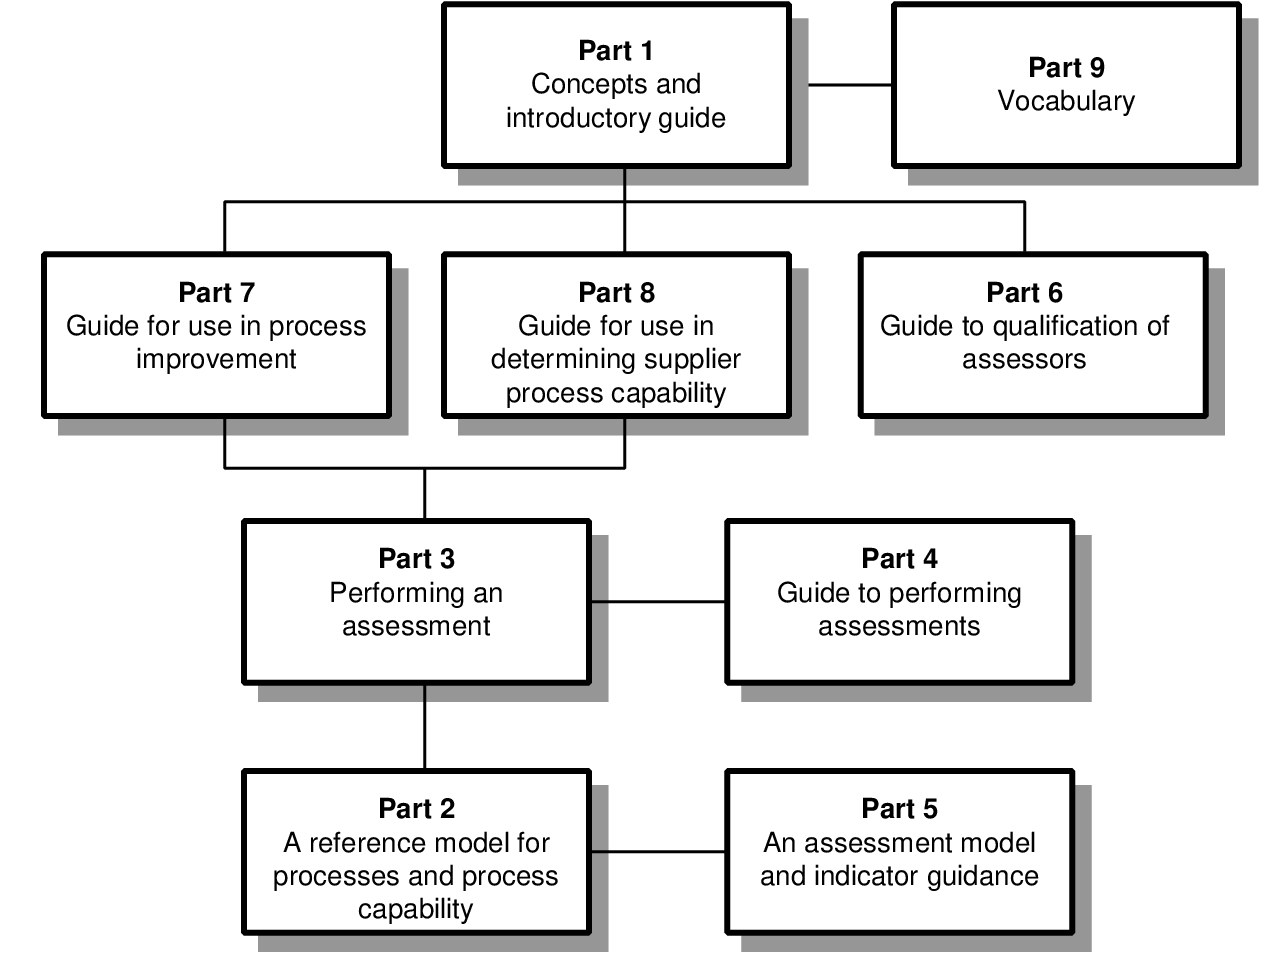
\includegraphics[width=10cm]{img/spice_doc.png}
    \label{fig:scice_documenti}
    \caption{Divisione documenti di SPICE}
\end{figure}


Nelle seguenti sezioni verranno descritte le caratteristiche principali dei documenti più significativi dello standard.

\subsubsection{Concetti iniziali}
\label{sub:concetti_iniziali}
Lo scopo del documento è fornite informazioni generali sulla valutazione del processo software e sul suo utilizzo in due contesti, miglioramento e determinazione della capacità del processo.
La determinazione della capacità del software è importante perchè generalmente motiva un'organizzazione a migliorare i processi.
In questo documento vengo inoltre spiegati i vantaggi che L'uso di SPICE fornisce a un'organizzazione, i più importanti vengono elencati di seguito:

\textbf{Per gli acquirenti}:
\begin{itemize}
    \item La possibilità di determinare la capacità attuale e potenziale dei processi software del fornitore.
\end{itemize}

\textbf{Per i fornitori}:
\begin{itemize}
    \item La possibilità di determinare la capacità attuale e potenziale dei propri processi software;
    \item La capacità di definire aree e priorità per il miglioramento dei processi software;
    \item Un framework che definisce una \glossario{ROAD MAP} per il miglioramento dei processi software.
\end{itemize}

\textbf{Per i valutatori}:
\begin{itemize}
    \item Un quadro che definisce gli aspetti dello svolgimento delle valutazioni.
\end{itemize}

\subsubsection{Modello di riferimento}
\label{sub:modello_di_riferimento}
Il documento fornisce una serie di pratiche fondamentali per una buona ingegneria del software.
Vengono definiti vari processi che possono essere utilizzati in varie fasi della produzione che possono essere raggruppati in cinque categorie che sono:

\begin{itemize}
    \item \textbf{Cliente-Fornitore}: sono processi che indicono direttamente sul cliente, supportano lo sviluppo e il passaggio del software cliente, garantendone il corretto funzionamento e utilizzo;
    \item \textbf{Ingegneria}: sono processi che specificano, implementano o gestiscono direttamente un prodotto software e di sistema e la relativa documentazione;
    \item \textbf{Progetto}: sono processi che servono a coordinare e gestire le risorse di un progetto;
    \item \textbf{Supporto}: sono processi che supportano le prestazione di altri processi;
    \item \textbf{Organizzazione}: sono processi che stabiliscono gli obiettivi di business dell'organizzazione che verranno raggiunti sviluppando processi, prodotti e risorse.
\end{itemize}

I processi vengono ulteriormente classificati in 6 livelli di capacità contenenti attributi per assegnare un valore quantificabile in modo da rendere esplicito come riuscire a migliorare tale processo.
I livelli definiti sono:
\begin{itemize}
    \item \textbf{0 - incompleto}: il processo è disordinato perché avente risultati e performance incomplete;
    \item \textbf{1 - Informale}: Il processo inizia ad essere eseguito con dati di input e output;
       \\ Attributi:
        \begin{itemize}
            \item \textbf{Esecuzione dei processi}: indica il numero di obiettivi raggiunti.
        \end{itemize}
    \item \textbf{2 - Gestito}: Sono definite le responsabilità e la gestione del processo;
        \\ Attributi:
        \begin{itemize}
            \item \textbf{Gestione del processo}: indica quanto sono organizzati gli obiettivi fissati;
            \item \textbf{Gestione del prodotto}: indica quanto sono organizzati o gestiti i prodotti rilasciati.
        \end{itemize}
    \item \textbf{3 - Stabilito}: Il processo è pronto per essere rilasciato diventando processo standard;
        \\ Attributi:
        \begin{itemize}
            \item \textbf{Definizione del processo}: indica quanto il processo aderisce agli standard;
            \item \textbf{Distribuzione del processo}: indica in che modo il processo possa essere rilasciato restituendo sempre lo stesso risultato.
        \end{itemize}
    \item \textbf{4 - Ben definito}: Il processo può essere sottoposto a metriche e valutazioni quantitative;
        \\ Attributi:
        \begin{itemize}
            \item \textbf{Misurazione del processo}: indica il numero di metriche che possono essere applicate al processo;
            \item \textbf{Controllo del processo}: Indica quanto i risultati delle previsioni sono predicibili.
        \end{itemize}
    \item \textbf{5 - Ottimizzante}: Il processo attua miglioramenti qualitativi e quantitativi.
        \\ Attributi:
        \begin{itemize}
            \item \textbf{Innovazione del processo}: indica, grazie a una fase di analisi, quanto i cambiamenti attuali del processo risultino positivi e innovativi;
            \item \textbf{Ottimizzazione del processo}: indica quanto la curva di miglioramento del processo sia lineare.
        \end{itemize}
\end{itemize}

Ad ogni attributo viene poi assegnata una valutazione in base alla sua percentuale di soddisfacimento:

\begin{itemize}
    \item \textbf{N}: il processo non svolge niente di significati e non è implementato (0\%-15\%);
    \item \textbf{P}: il processo è implementato parzialmente (15\%-50\%);
    \item \textbf{L}: il processo è largamente implementato (50\%-85\%);
    \item \textbf{F}: il processo è completamente implementato (85\%-100\%).
\end{itemize}


\subsubsection{Valutazioni}
\label{sub:valutazioni}
Il documento prosegue fornendo una guida per eseguire una valutazione che comprende:
\begin{itemize}
    \item Il processo di valutazione;
    \item Il modello di valutazione;
    \item Eventuali strumenti utilizzati nella valutazione;
\end{itemize}

\paragraph{Processo di valutazione}
\label{sub:processo_di_valutazione}
Uno dei requisiti del documento è utilizzare un metodo di valutazione conforme per il processo di valutazione.
Il processo di valutazione può essere generalizzato nei seguenti passaggi:
\begin{itemize}
    \item Avviare una valutazione;
    \item Selezionare il valutatore e il gruppo di valutazione;
    \item Pianificare la valutazione, compresi i processi e le unità organizzative da valutare;
    \item Eseguire un \glossario{BRIEFING} prima di avviare la valutazione;
    \item Raccogliere i dati;
    \item Validare i dati;
    \item Valutare il processo attraverso un rating;
    \item Riportare il risultato della valutazione.
\end{itemize}

\paragraph{Modello di valutazione}
\label{sub:modello_di_valutazione}
Il modello di valutazione del processo (PAM) è il modello dettagliato utilizzato per una valutazione effettiva.
Nella parte 5 il modello di riferimento del processo per il software è ISO/IEC 12207 mentre nella parte 6 il modello di riferimento del processo per i sistemi è ISO/IEC 15288.
Lo standard consente di utilizzare altri modelli purché soddisfino i criteri di ISO/IEC 15504.

\paragraph{Strumenti di valutazione}
\label{sub:strumenti_di_valutazione}
Esistono diversi strumenti di valutazione, i più semplici comprendono strumenti cartacei. In generale, sono previsti per incorporare gli indicatori del modello di valutazione, inclusi gli indicatori di pratica di base e gli indicatori di pratica generica. I valutatori scrivono i risultati della valutazione e le note a supporto del giudizio di valutazione.
Per quanto riguarda gli strumenti basati su software sono in numero limitato pertanto sono preferibili gli strumenti in modalità cartacea.

\subsection{ISO/IEC 9126}%
\label{sec:iso/iec_9126}
ISO/EIC 9126 è uno standard che definisce in modello di qualità del software. Il modello propone un approccio alla qualità con lo scopo di migliorare l'organizzazione e i processi di una società di software, migliorando di conseguenza la qualità del prodotto.
Lo standard descrive un modello di qualità diviso in 3 parti:
\begin{itemize}
    \item \textbf{Qualità interna}: si applica al software non eseguibile (come il codice sorgente) durante le fasi di progettazione e codifica.
    Le misure in questa fase permettono di prevedere anche i livelli di qualità esterna e in uso del prodotto dato che essi dipendono dalla qualità interna.
    Per misurare la qualità interna vengono utilizzate le metriche interne che permettono di individuare eventuali problemi attraverso l'analisi statica e la simulazione del comportamento del prodotto finale tramite delle simulazioni;
    \\Gli attributi che possono essere assegnati alla qualità interna sono:
    \begin{itemize}
        \item Manutenibilità;
        \item Portabilità.
    \end{itemize}
    \item \textbf{Qualità esterna}: viene applicata al software durante la sua esecuzione, utilizza le metriche esterne per misurare i comportamenti del software sulla base di test, dell'operatività e dall'osservazione durante l'esecuzione di essi;
    \\Gli attributi assegnati ad essa sono:
    \begin{itemize}
        \item Funzionalità;
        \item Efficienza;
        \item Affidabilità;
        \item Usabilità.
    \end{itemize}
    \item \textbf{Qualità d'uso}: rappresenta il punto di vista dell'utente sul software ed è fortemente influenzata dalle precedenti 2 qualità. Essa permette di abilitare specifici utenti ad ottenere specifici obiettivi sui suoi relativi attributi.
    \\Gli attributi assegnati ad essa sono:
    \begin{itemize}
        \item Efficacia;
        \item Produttività;
        \item Soddisfazione;
        \item Sicurezza.
    \end{itemize}
\end{itemize}
Ovviamente per ciascun attributo delle tre qualità è misurabile e valutabile secondo le relative metriche: interne, esterne e d'uso.

\begin{figure}[H]
    \centering
    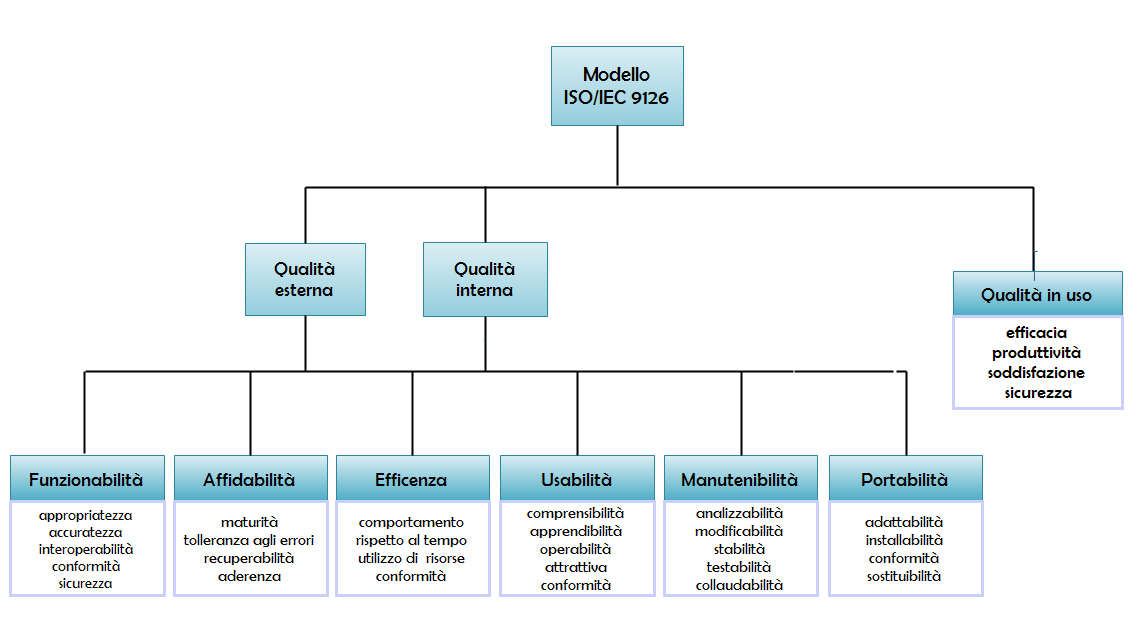
\includegraphics[width=10cm]{img/Modello_ISO-IEC_9126.png}
    \label{fig:modello_iso_eic_9126}
    \caption{Modello ISO/IEC 9126}
\end{figure}

\subsubsection{Descrizione degli attributi di Qualità interni ed esterni}%
\label{sec:descrizione_attributi_interni_esterni}
Verranno descritti brevemente ciascun attributo relativo alla Qualità interna e alla Qualità esterna, per ogni attributo verranno analizzate le sue sottocaratteristiche.

\begin{itemize}
    \item \textbf{Manutenibilità}: il software deve essere facilmente modificabile nel caso di correzioni, adattamenti e/o miglioramenti.
        \\Per le sue sottocaratteristiche sono previste:
        \begin{itemize}
            \item \textbf{Analizzabilità}: il software deve essere facilmente leggibile in modo da trovare facilmente eventuali errori;
            \item \textbf{Modificabilità}: il software deve essere estendibile con modifiche precise;
            \item \textbf{Stabilità}: il software deve rimanere stabile in caso di modifiche errate;
            \item \textbf{Testabilità}: il software deve essere facilmente testabile in modo da validare le modifiche effettuate.
        \end{itemize}
        \item \textbf{Portabilità}: il software dovrebbe essere facilmente portabile ed eseguibile in diversi ambienti.
        \\Per le sue sottocaratteristiche sono previste:
        \begin{itemize}
            \item \textbf{Adattabilità}: il software deve adattarsi a diversi ambienti senza necessità di apportare modifiche;
            \item \textbf{Installabilità}: il software deve essere facilmente installabile;
            \item \textbf{Conformità}: il software deve coesistere con altre applicazioni e deve essere coerente con gli standard e le norme richieste della portabilità;
            \item \textbf{Sostituibilità}: il software deve essere in grado di sostituire un altro software adempiendo agli stessi scopi.
        \end{itemize}
        \item \textbf{Funzionalità}: il software deve fornire funzioni che soddisfino le esigenze stabilite in base all'ambiente d'esecuzione;
        \\Per le sue sottocaratteristiche sono previste:
        \begin{itemize}
            \item \textbf{Appropriatezza}: il software deve fornire un appropriato insieme di funzioni per i compiti richiesti;
            \item \textbf{Accuratezza}: il software deve fornire gli effetti richiesti;
            \item \textbf{Interoperabilità}: il software deve essere in grado di operare con uno o più sistemi specifici;
            \item \textbf{Conformità}: il software deve aderire agli standard e alle norme richieste dal settore;
            \item \textbf{Sicurezza}: il software deve essere in grado di proteggere le proprie informazioni da agenti esterni.
        \end{itemize}
        \item \textbf{Efficienza}: il software deve fornire le giuste prestazioni in base alla proprie risorse;
        \\Per le sue sottocaratteristiche sono previste:
        \begin{itemize}
            \item \textbf{Comportamento rispetto al tempo}: il software deve adeguati tempi di elaborazione e risposta sotto determinate condizioni;
            \item \textbf{Utilizzo delle risorse}: il software deve utilizzare le risorse in modo adeguato;
            \item \textbf{Conformità}: il software deve aderire agli standard di efficienza richiesti.
        \end{itemize}
        \item \textbf{Affidabilità}: il software deve mantenere un certo livello di prestazioni quando usato in certe condizioni;
        \\Per le sue sottocaratteristiche sono previste:
        \begin{itemize}
            \item \textbf{Maturità}: il software non deve produrre errori , malfunzionamenti o risultati non aspettati;
            \item \textbf{Tolleranza agli errori}: il software deve mantenere le prestazioni anche in presenza di malfunzionamenti;
            \item \textbf{Recuperabilità}: il software deve essere in grado di ripristinare le prestazioni dopo un malfunzionamento, nel minor tempo possibile;
            \item \textbf{Aderenza}:il software deve aderire alle regole e convenzioni sull'affidabilità;
        \end{itemize}
        \item \textbf{Usabilità}: il software deve essere facilmente capito e usato dagli utenti.
        \begin{itemize}
            \item \textbf{Comprensibilità}: il codice deve esprimere concetti semplici e chiari per l'uso da parte dell'utente;
            \item \textbf{Apprendibilità}: il software non deve richiedere troppo tempo agli utenti per imparare ad usarlo;
            \item \textbf{Operabilità}: il software deve poter mettere gli utenti in condizione di farne un uso per i propri scopi;
            \item \textbf{Attrattivà}: il software deve piacere agli utenti;
            \item \textbf{Conformità}: il software deve aderire agli standard di usabilità.
        \end{itemize}
\end{itemize}


\subsubsection{Descrizione degli attributi di Qualità in uso}%
\label{sec:descrizione_attributi_in_uso}
Verranno descritti brevemente ciascun attributo relativo alla Qualità in suo.

Attributi
\begin{itemize}
    \item \textbf{Efficacia}: capacità del software di mettere in grado gli utenti di raggiungere i propri obiettivi con accuratezza e completezza;
    \item \textbf{Produttività}: capacità per gli utenti di utilizzare le risorse appropriate, in relazione all'efficacia, per ottenere un contesto specificato;
    \item \textbf{Soddisfazione}: capacità del prodotto di soddisfare gli utenti;
    \item \textbf{Sicurezza}: capacità del software di raggiungere certi livelli di riservatezza;
\end{itemize}

\subsection{Ciclo di Deming}%
\label{sec:ciclo_di_deming}
Il Ciclo di Deming è un metodo iterativo utilizzato per il controllo e il miglioramento continuo della qualità dei processi e dei prodotti.
Serve per promuovere una cultura della qualità che si basa sul miglioramento continuo dei processi e sull'ottimizzazione delle risorse.
Questo strumento ha come scopo il raggiungimento del massimo della qualità mediante la costante iterazione tra ricerca,progettazione,test,produzione e vendita, ed è necessario passare in tutte le fasi per soddisfare la qualità richiesta dal cliente.

Il ciclo è anche chiamato PDCA in riferimento alla sua divisione in 4 fasi:
\begin{itemize}
    \item \textbf{P - Plan} Pianificazione: stabilire obiettivi e processi necessari per ottenere i risultati attesi e capire dove questi possono essere migliorati;
    \item \textbf{D - Do} Esecuzione del programma: eseguire il programma stilato nella fase precedente, raccogliere dati per la creazione di analisi per le successive fasi di "Check" e "Act";
    \item \textbf{C - Check} Test e controllo: studio dei dati raccolti e confrontarli con i risultati attesi nella fase di "Plan". Valutare i risultati e verificare se i cambiamenti attuati possono portare a miglioramenti;
    \item \textbf{A - Act} Azione: Richiede azioni correttive sulle differenze tra i risultati previsti e quelli effettivi, analizza le differenze per determinare dove applicare le modifiche per ottenere un miglioramento del prodotto o processo.
\end{itemize}
Quando un procedimento attraversa le quattro fasi, non è obbligato a migliorare immediatamente, il ciclo può essere ripetuto tutto o in parte per raffinare maggiormente il prodotto.
\\ \\
\begin{figure}[H]
    \centering
    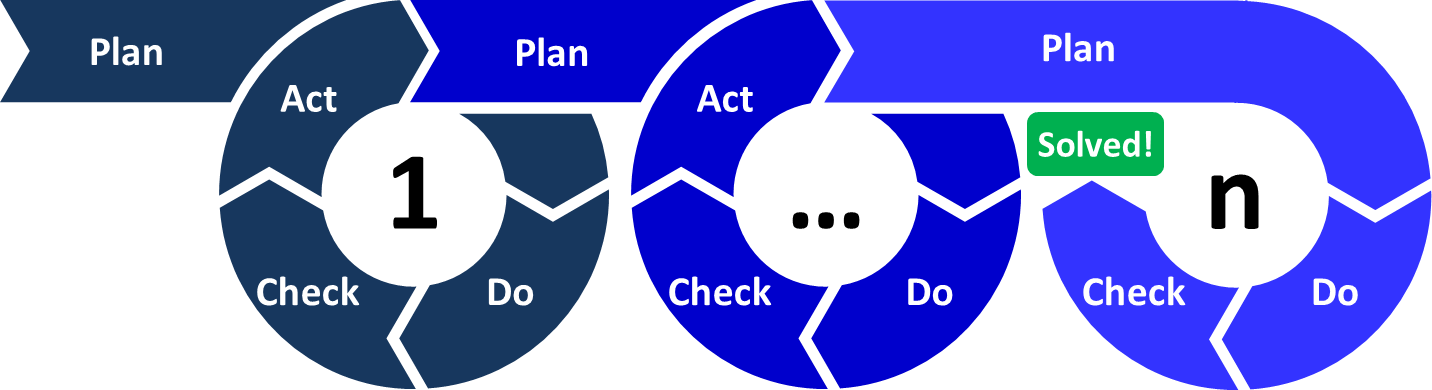
\includegraphics[width=10cm]{img/ciclo_di_deming.png}
    \label{fig:ciclo_di_deming}
    \caption{Ciclo di Deming}
\end{figure}

\end{document}